\documentclass[a4paper]{article}
% Этот шаблон документа разработан в 2014 году
% Данилом Фёдоровых (danil@fedorovykh.ru) 
% для использования в курсе 
% <<Документы и презентации в \LaTeX>>, записанном НИУ ВШЭ
% для Coursera.org: http://coursera.org/course/latex .
% Исходная версия шаблона --- 
% https://www.writelatex.com/coursera/latex/5.3

% В этом документе преамбула

\usepackage{siunitx}
%%% Работа с русским языком
%\usepackage{cmap}					% поиск в PDF
%\usepackage{mathtext} 				% русские буквы в формулах
%\usepackage[T2A]{fontenc}			% кодировка
%\usepackage[utf8]{inputenc}			% кодировка исходного текста
%\usepackage[english,russian]{babel}	% локализация и переносы
%\usepackage{indentfirst}
%\frenchspacing
%
%\renewcommand{\epsilon}{\ensuremath{\varepsilon}}
%\newcommand{\phibackup}{\ensuremath{\phi}}
%\renewcommand{\phi}{\ensuremath{\varphi}}
%\renewcommand{\varphi}{\ensuremath{\phibackup}}
%\renewcommand{\kappa}{\ensuremath{\varkappa}}
%\renewcommand{\le}{\ensuremath{\leqslant}}
%\renewcommand{\leq}{\ensuremath{\leqslant}}
%\renewcommand{\ge}{\ensuremath{\geqslant}}
%\renewcommand{\geq}{\ensuremath{\geqslant}}
%\renewcommand{\emptyset}{\varnothing}
%\renewcommand{\Im}{\operatorname{Im}}
%\renewcommand{\Re}{\operatorname{Re}}


%%% Дополнительная работа с математикой
\usepackage{amsmath,amsfonts,amssymb,amsthm,mathtools} % AMS
%\usepackage{icomma} % "Умная" запятая: $0,2$ --- число, $0, 2$ --- перечисление

%% Номера формул
%\mathtoolsset{showonlyrefs=true} % Показывать номера только у тех формул, на которые есть \eqref{} в тексте.
%\usepackage{leqno} % Нумереация формул слева

%% Свои команды
\DeclareMathOperator{\sgn}{\mathop{sgn}}
\DeclareMathOperator{\sign}{\mathop{sign}}
\DeclareMathOperator*{\res}{\mathop{res}}
\DeclareMathOperator*{\tr}{\mathop{tr}}
\DeclareMathOperator*{\rot}{\mathop{rot}}
\DeclareMathOperator*{\divop}{\mathop{div}}
\DeclareMathOperator*{\grad}{\mathop{grad}}

%% Перенос знаков в формулах (по Львовскому)
\newcommand*{\hm}[1]{#1\nobreak\discretionary{}
{\hbox{$\mathsurround=0pt #1$}}{}}

%%% Работа с картинками
\usepackage{graphicx}  % Для вставки рисунков
\graphicspath{{figures/}}  % папки с картинками
\setlength\fboxsep{3pt} % Отступ рамки \fbox{} от рисунка
\setlength\fboxrule{1pt} % Толщина линий рамки \fbox{}
\usepackage{wrapfig} % Обтекание рисунков текстом

%%% Работа с таблицами
\usepackage{array,tabularx,tabulary,booktabs} % Дополнительная работа с таблицами
\usepackage{longtable}  % Длинные таблицы
\usepackage{multirow} % Слияние строк в таблице

%%% Теоремы
\theoremstyle{plain} % Это стиль по умолчанию, его можно не переопределять.
\newtheorem{thm}{Теорема}
\newtheorem*{thm*}{Теорема}
\newtheorem{prop}{Предложение}
\newtheorem*{prop*}{Предложение}
 
\theoremstyle{definition} % "Определение"
%\newtheorem{corollary}{Следствие}[theorem]
\newtheorem{dfn}{Определение}
\newtheorem*{dfn*}{Определение}
\newtheorem{prob}{Задача}
\newtheorem*{prob*}{Задача}

 
\theoremstyle{remark} % "Примечание"
\newtheorem*{sol}{Решение}
\newtheorem*{rem}{Замечание}

%%% Программирование
\usepackage{etoolbox} % логические операторы

%%% Страница
%\usepackage{extsizes} % Возможность сделать 14-й шрифт
%\usepackage{geometry} % Простой способ задавать поля
%	\geometry{top=25mm}
%	\geometry{bottom=35mm}
%	\geometry{left=35mm}
%	\geometry{right=20mm}
 
\usepackage{fancyhdr} % Колонтитулы
%	\pagestyle{fancy}
 %	\renewcommand{\headrulewidth}{0pt}  % Толщина линейки, отчеркивающей верхний колонтитул
	%\lfoot{Нижний левый}
	%\rfoot{Нижний правый}
	%\rhead{Верхний правый}
	%\chead{Верхний в центре}
	%\lhead{Верхний левый}
	%\cfoot{Нижний в центре} % По умолчанию здесь номер страницы

\usepackage{setspace} % Интерлиньяж
%\onehalfspacing % Интерлиньяж 1.5
%\doublespacing % Интерлиньяж 2
%\singlespacing % Интерлиньяж 1

\usepackage{lastpage} % Узнать, сколько всего страниц в документе.

\usepackage{soul} % Модификаторы начертания

\usepackage{hyperref}
\usepackage[usenames,dvipsnames,svgnames,table,rgb]{xcolor}
\hypersetup{				% Гиперссылки
    unicode=true,           % русские буквы в раздела PDF
    pdftitle={Заголовок},   % Заголовок
    pdfauthor={Автор},      % Автор
    pdfsubject={Тема},      % Тема
    pdfcreator={Создатель}, % Создатель
    pdfproducer={Производитель}, % Производитель
    pdfkeywords={keyword1} {key2} {key3}, % Ключевые слова
%    colorlinks=true,       	% false: ссылки в рамках; true: цветные ссылки
    %linkcolor=red,          % внутренние ссылки
    %citecolor=black,        % на библиографию
    %filecolor=magenta,      % на файлы
    %urlcolor=cyan           % на URL
}

\usepackage{csquotes} % Еще инструменты для ссылок

%\usepackage[style=apa,maxcitenames=2,backend=biber,sorting=nty]{biblatex}

\usepackage{multicol} % Несколько колонок

\usepackage{tikz} % Работа с графикой
\usepackage{pgfplots}
\usepackage{pgfplotstable}
%\usepackage{coloremoji}
\usepackage{floatrow}
\usepackage{subcaption}
\graphicspath{{figures/}}

\renewcommand\thesubfigure{\asbuk{subfigure}}
%\addbibresource{master.bib}

\usepackage{import}
\usepackage{pdfpages}
\usepackage{transparent}
\usepackage{xcolor}
\usepackage{xifthen}

\newcommand{\incfig}[2][1]{%
    \def\svgwidth{#1\columnwidth}
    \import{./figures/}{#2.pdf_tex}
}
%\usepackage{titlesec}
%\titleformat{\section}{\normalfont\Large\bfseries}{}{0pt}{}
%----------------------STANDART:
%\titleformat{\chapter}[display]
%  {\normalfont\huge\bfseries}{\chaptertitlename\ \thechapter}{20pt}{\Huge}
%\titleformat{\section}{\normalfont\Large\bfseries}{\thesection}{1em}{}
%\titleformat{\subsection}
%  {\normalfont\large\bfseries}{\thesubsection}{1em}{}
%\titleformat{\subsubsection}
%  {\normalfont\normalsize\bfseries}{\thesubsubsection}{1em}{}
%\titleformat{\paragraph}[runin]
%  {\normalfont\normalsize\bfseries}{\theparagraph}{1em}{}
%\titleformat{\subparagraph}[runin]
%  {\normalfont\normalsize\bfseries}{\thesubparagraph}{1em}{}

\pdfsuppresswarningpagegroup=1
\pgfplotsset{compat=1.16}



%\setcounter{tocdepth}{1} % only parts,chapters,sections
%\titleformat{\subsection}{\normalfont\large\bfseries}{}{0em}{}
%\titleformat{\subsubsection}{\normalfont\normalsize\bfseries}{}{0em}{}

%\newcommand{\textover}[2]{\stackrel{\mathclap{\normalfont\mbox{#2}}}{#1}}

\author{Yaroslav Drachov\\
Moscow Institute of Physics and Technology}
%\author{Драчов Ярослав\\
%Факультет общей и прикладной физики МФТИ}
\newcommand{\veq}{\mathrel{\rotatebox{90}{$=$}}}
%\newcommand{\teto}[1]{\stackrel{\mathclap{\normalfont\tiny\mbox{#1}}}{\to}}
%\renewcommand{\thesubsection}{\arabic{subsection}}

%%\setcounter{secnumdepth}{0}

\definecolor{tabblue}{RGB}{30, 119, 180}
\definecolor{taborange}{RGB}{255, 127, 15}
\definecolor{tabgreen}{RGB}{45, 160, 43}
\definecolor{tabred}{RGB}{214, 38, 40}
\definecolor{tabpurple}{RGB}{148, 103, 189}
\definecolor{tabbrown}{RGB}{140, 86, 76}
\definecolor{tabpink}{RGB}{227, 119, 193}
\definecolor{tabgray}{RGB}{127, 127, 127}
\definecolor{tabolive}{RGB}{188, 189, 33}
\definecolor{tabcyan}{RGB}{22, 190, 207}
\pgfplotscreateplotcyclelist{colorbrewer-tab}{
{tabblue},
{taborange},
{tabgreen},
{tabred},
{tabpurple},
{tabbrown},
{tabpink},
{tabgray},
{tabolive},
{tabcyan},
}
\usepackage{csvsimple}
\usepackage{extarrows}
%\renewcommand{\labelenumii}{\asbuk{enumii})}
%\renewcommand{\labelenumiv}{\Asbuk{enumiv}}
%\newcommand{\prob}[1]{\subsubsection*{#1}}
\sisetup{output-decimal-marker = {,},separate-uncertainty = true,exponent-product = \cdot}

\usepackage{braket}
\usepackage{enumerate}
\usepackage{chngcntr}
%\counterwithin*{equation}{problem}
%\usepackage{bbold}

\newtheoremstyle{hiProb}% ⟨name ⟩ 
{3pt}% ⟨Space above ⟩1 
{3pt}% ⟨Space below ⟩1
{}% ⟨Body font ⟩
{}% ⟨Indent amount ⟩2
{\bfseries}% ⟨Theorem head font⟩
{.}% ⟨Punctuation after theorem head ⟩
{.5em}% ⟨Space after theorem head ⟩3
%{\thmname{#1} \thmnote{#3}}% ⟨Theorem head spec (can be left empty, meaning ‘normal’)⟩
{\thmnote{#3}}% ⟨Theorem head spec (can be left empty, meaning ‘normal’)⟩
\theoremstyle{hiProb} % "Определение"
%\newtheorem{hiProb}{Задача}
\newtheorem{hiProb}{}
%\usepackage{mmacells}
\newcommand{\textover}[2]{\stackrel{\mathclap{\normalfont\scriptsize\mbox{#2}}}{#1}}
\usepackage{units}
\usepackage[math]{cellspace}%
\setlength\cellspacetoplimit{2pt}
\setlength\cellspacebottomlimit{2pt}

\DeclareMathAlphabet{\mathbbold}{U}{bbold}{m}{n}

\newcommand{\normord}[1]{:\mathrel{#1}:}

\title{Лабораторная работа №11.5\\
Туннелирование в проводниках}
\begin{document}
	\maketitle

	\paragraph*{Цель работы:} исследовать принцип действия туннельного диода, измерить его вольт-амперную характеристику и основные параметры. 
	
	
	
	\section{Теоретическое введение}
	
	Туннельным диодом называется сильно легированный полупроводник, уровень Ферми которого лежит в разрешенной зоне и становятся возможны туннельные переходы электронов в области узкого $(p-n)$-перехода. 
	
	Будем считать, что все состояния, лежащие ниже уровня Ферми, заполнены электроны, а выше --- свободны. Энергетические диаграммы идеального туннельного диода и его вольт-амперная характеристика показаны на рисунке \ref{pic:diode}. $\mu_n$ и $\mu_p$ обозначены уровни Ферми в $n$- и $p$-области соответственно; $E_c$ и $E_v$ - границы зоны проводимости и валентной зоны. В отсутсвии внешнего поля уровни Ферми $\mu_n$ и $\mu_p$ лежат на одной горизонтали; число дырок и электронов, туннелирующих в обе стороны, одинаково, и ток отсутствует (рисунок \ref{pic:diode}.\textit{a}). При приложении напряжения в прямом направлении уровень Ферми в $n$-области <<ползет>> вверх по отношению к уровню Ферми в $p$-области, электроны туннелируют налево, ток растет. Он достигает максимума в точке \textit{б} вольт-амперной характеристики (рисунок \ref{pic:diode}.\textit{ж}), соответствующей наибольшему совпадению занятой зоны в отрицательной области и свободной в положительной. При дальнейшем увеличении внешнего напряжения перекрытие занятых уровней в $n$-области и свободных в $p$- уменьшается, и ток падает до нуля: это иллюстрирует рисунок \ref{pic:diode}.\textit{в}. Предельное положение соответствует энергетической диаграмме \textit{г}. При дальнейшем увеличении напряжения ток, возникающий за счет туннелирующих электронов, остается равным нулю, а диффузиозный ток возникает при совпадении занятых уровней $n$-области с свободными уровнями зоны проводимости (рисунок \ref{pic:diode}.\textit{д}). На диаграмме \ref{pic:diode}.\textit{е} показан ток в обратном направлении. 
	
	\begin{figure}[h]
		\centering	
		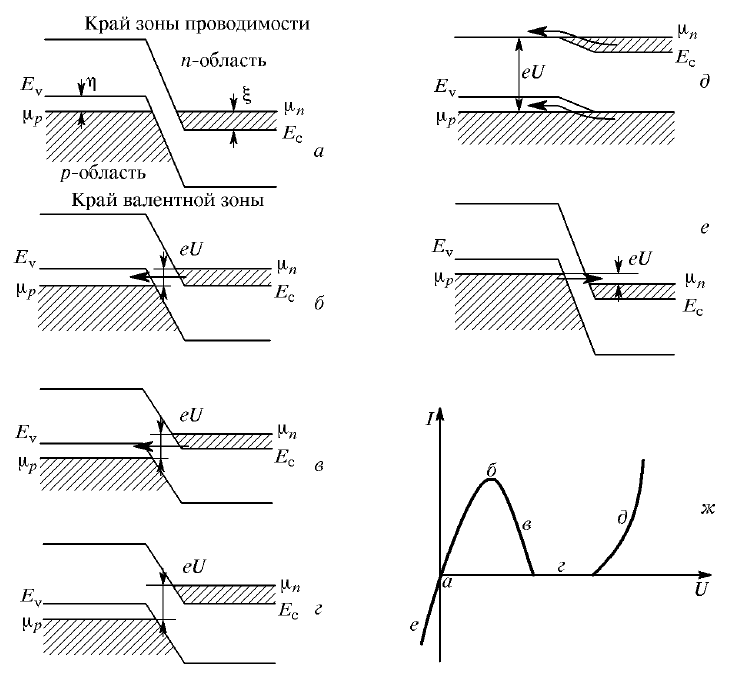
\includegraphics[width=0.5\textwidth]{diode.png}
		\caption{Схема энергетических уровней и вольт-амперная характеристика идеального туннельного диода}
		\label{pic:diode}
	\end{figure}  
	
	Реальная вольт-амперная характеристика туннельного диода отличается от таковой для идеального и представлена на рисунке \ref{pic:not_ideal}. Она учитывает образование примесных зон и возможность их слияния с основными, что объясняет наличия ненулевого тока $I_v$ в минимуме характеристики. 
	
	\begin{figure}[h]
		\centering	
		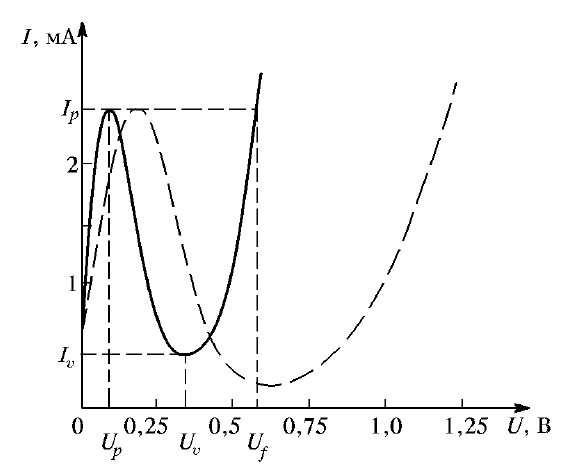
\includegraphics[width=0.4\textwidth]{not_ideal.png}
		\caption{Вольт-амперная характеристика неидеальных туннельных диодов с меньшей (сплошная линия) и большей (пунктирная линия) шириной запрещенной зоны}
		\label{pic:not_ideal}
	\end{figure}  
	
	Вольт-амперная характеристика реального туннельного диода (см. рисунок \ref{pic:not_ideal}) описывается следующими значениями напряжения и тока. 
	
	Напряжению $U_p$ соответствует максимум тока $I_p$, при котором смещение энергетических зон одинаково, причем это напряжение связано с расстоянием $\xi$ между уровнем Ферми в $n$-области и зоной проводимости и энергией $E_\text{n max}$, соответствующей максимуму плотности распределения электронов, следующим отношением: 
	
	\[ U_p \approx \frac{\xi - E_\text{n max}}{e} \]
	
	В точке $U_v$ ток минимален, и, как следует из описания выше:
	
	\[ U_v \approx \frac{(\mu_n - E_c) + (E_v - \mu_p)}{e} = \frac{\xi + \eta}{e} \approx \frac{2\xi}{e} \approx \frac{2\eta}{e} \]
	
	Напряжение $U_f$ характеризует раствор вольт-амперной характеристики и определяется шириной запрещенной зоны. 


	\section{Изучение вольт-амперной характеристики диода с помощью осциллографа}
	
	Схема установки представлена на рисунке \ref{pic:scheme_oscil}. На вход $ Y $ осциллографа подается напряжение, пропорциональное току через диод, а на вход $ X $ --- падение напряжения на диоде.
	
	\begin{figure}[h]
		\centering	
		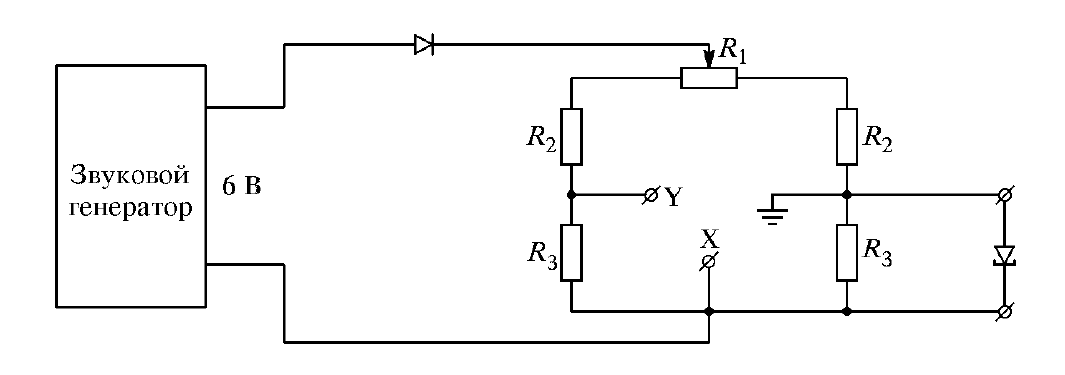
\includegraphics[width=0.5\textwidth]{scheme_oscil.png}
		\caption{Схема наблюдения вольт-амперной характеристики туннельного диода с помощью осциллографа}
		\label{pic:scheme_oscil}
	\end{figure}
	
	Ток $I$ через диод зависит от напряжения $U$ на нем по следующей формуле: 
	
	\[ I = U \frac{R_1 + 2(R_2 + R_3)}{(R_1 + 2R_2) \cdot R_3} \]
	
	Здесь $R_1$, $R_2$, $R_3$ --- сопротивления соответствующих резисторов моста со схемы на рисунке \ref{pic:scheme_oscil}. 

Вольт-амперная характреристика исследуемого проводникового диода на экране осциллографа представлена на рис.~\ref{fig:2}. По оси X
масштаб 50 мВ, значит $U_p \approx 50  $ мВ, $U_v \approx 300$ мВ,
$U_f \approx 400$ мВ, $I_v\approx 0,2$ мА, $I_p \approx 2$ мА.
\begin{figure}[htpb]
	\centering
	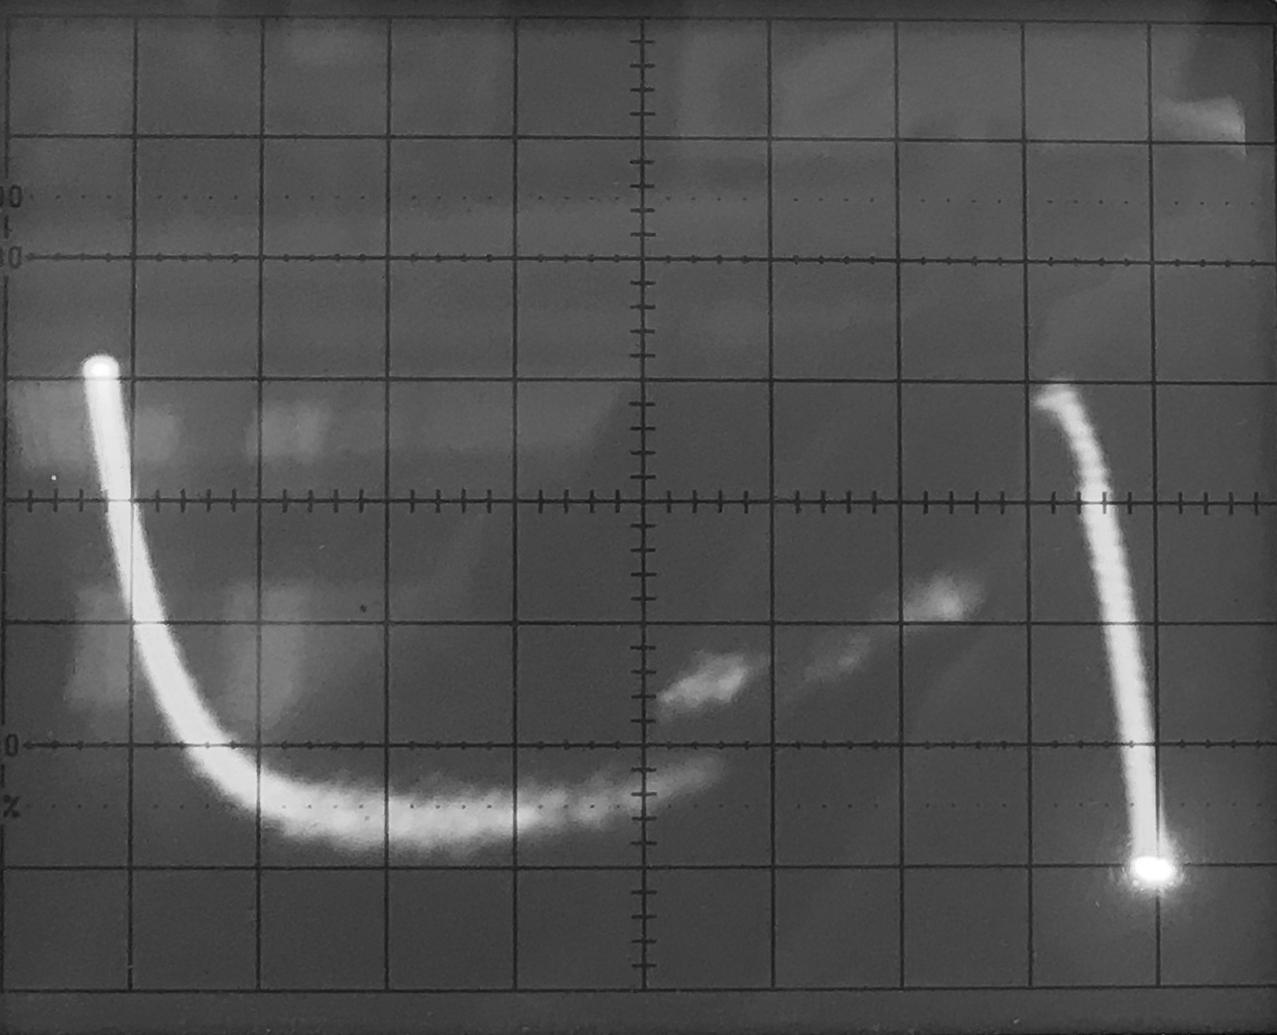
\includegraphics[width=0.8\textwidth]{2}
	\caption{ВАХ в динамическом режиме}
	\label{fig:2}
\end{figure}
Со статической ВАХ на рис.~\ref{fig:1} можно уточнить полученные
результаты:
\[
U_p= 34,9\pm 0,6 \text{ мВ},\quad I_p=1,963\pm 0,009 \text{ мА}
 ,\]
\[
U_v=0,29 \pm 0,02 \text{ В},\quad I_v=0,191\pm 0,007 \text{ мА}
,\] 
\[
U_f=436\pm 3 \text{ мВ}
.\] 
\begin{figure}[htpb]
	\centering
	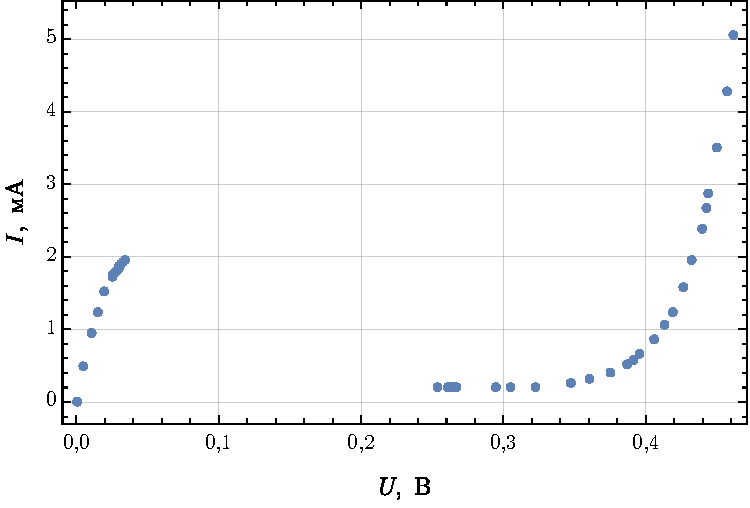
\includegraphics[width=0.8\textwidth]{1}
	\caption{ВАХ в статическом режиме}
	\label{fig:1}
\end{figure}
Примем $E_v=0$. Тогда из выражения для $U_v\approx 2\mu e$ 
можно найти энергию Ферми $\mu_n \approx \mu_p$:
\[
\mu_n \approx \mu_p \approx e U_v /2=0,15\pm 0,01 \text{ эВ}
.\] 
Из выражения для напряжения $U_p\approx (\mu_n -E_{n \text{ max}}) /e$ получим энергию, соответствующую максимальной
плотности распределения электронов $E_{n \text{ max}}$:
\[
E_{n \text{  max}}=\mu_n-eU_p= 0,12\pm 0,01 \text{ эВ}
.\] 
В ходе изучения генератора на основе туннельного диода
было выяснено, что частота генерации для амплитуд от
0.1 до 0.4 В остаётся постоянной.
	\section{Вывод} 
	В работе исследован принцип действия туннельного диода; мы наблюдали его вольт-амперную характеристику на осциллографе и затем измерили ее непосредственно, снимая зависимость тока от напряжения. 
	
	По результатам измерений мы получили параметры диода, которые совпадают с грубой оценкой, полученной благодаря наблюдению на осциллографе.
	\begin{table}[htpb]
		\centering
		\caption{Измерения}
		\label{tab:1}
		\csvreader[tabular=|c|c|,
		table head={\hline $U$, В & $I$, мА \\\hline},
		late after line=\\\hline, head to column names]
		{datasethi.csv}{}
		{\U & \I}
	\end{table}
\end{document}
